% Компіляція: lualatex -shell-escape main.tex (двічі)
\documentclass[12pt,a4paper]{article}

\usepackage{fontspec}
\usepackage{polyglossia}
\setdefaultlanguage{ukrainian}
\setmainfont{NewComputerModern10}
\setsansfont{Noto Sans}
\setmonofont{Noto Sans Mono}[Scale=0.82]

\usepackage{
  amsmath,
  amssymb,
  array,
  booktabs,
  caption,
  enumitem,
  float,
  geometry,
  graphicx,
  microtype,
  titlesec,
  xcolor
}
\usepackage{tikz}
\usetikzlibrary{arrows.meta,positioning,shapes.geometric}
\geometry{left=2cm,right=2cm,top=2cm,bottom=2cm}
\setlength{\parindent}{1.25cm}
\setlength{\parskip}{0pt}
\linespread{1.08}
\titleformat{\section}
  {\normalfont\fontsize{14}{16}\selectfont\bfseries}
  {\thesection}{0.6em}{}
\titleformat{\subsection}
  {\normalfont\fontsize{12}{14}\selectfont\bfseries}
  {\thesubsection}{0.6em}{}
\titlespacing*{\section}{0pt}{1.4em}{0.65em}
\titlespacing*{\subsection}{0pt}{1.1em}{0.45em}
\captionsetup{font=small,labelfont=bf,labelsep=endash}
\captionsetup[table]{position=bottom,skip=5pt}
\setlist{itemsep=2pt,topsep=4pt}

\usepackage[newfloat]{minted}
\SetupFloatingEnvironment{listing}{name=Лістинг}
\setminted{
  fontsize=\scriptsize,
  linenos,
  breaklines,
  breakanywhere,
  autogobble,
  frame=single,
  framesep=2mm,
  bgcolor=gray!5,
  tabsize=4
}

\usepackage[
  unicode,
  colorlinks=true,
  linkcolor=black,
  urlcolor=blue,
  pdftitle={ІО-41, Давидчук Артем, Інформаційне забезпечення промислових роботів, Лабораторна робота №4},
  pdfauthor={Давидчук Артем},
  pdfsubject={Сенсори та приводи мобільних роботів}
]{hyperref}

\begin{document}

\pagenumbering{gobble}
\begin{titlepage}
  \begin{center}
    
\includegraphics[width=0.7\textwidth]{../../../../../templates/letterhead.png}
  \end{center}

  \begin{center}
    \large
    Національний технічний університет України\\
    «Київський політехнічний інститут імені Ігоря Сікорського»\\[1em]
    Факультет інформатики та обчислювальної техніки\\
    Кафедра обчислювальної техніки
  \end{center}

  \vfill

  \begin{center}
    \textbf{\LARGE Інформаційне забезпечення\\промислових роботів}\\[2em]
    \textbf{\Large Лабораторна робота №4}\\[0.7em]
    \parbox{0.9\textwidth}{\centering
      «Сенсори та приводи мобільних роботів»}
  \end{center}

  \vfill

  \begin{flushright}
    \begin{minipage}{0.48\textwidth}
      Виконав: студент групи ІО-41\\
      \textit{Давидчук Артем}\\
      \\[1em]
      Перевірив: \textit{Тюляков Дмитро Ігорович}
    \end{minipage}
  \end{flushright}

  \vfill

  \begin{center}Київ --- 2026\end{center}
\end{titlepage}
\pagenumbering{arabic}

\section{Мета роботи}

Ознайомитися з датчиками й приводами мобільних роботів та реалізувати
замкнений алгоритм автономного руху групи колісних роботів у середовищі
\textit{CoppeliaSim Edu}.

\section{Постановка задачі}

У сцені розміщено п'ять роботів \texttt{Pioneer P3-DX}, стіни арени та
циліндричні перешкоди. Для кожного робота потрібно отримувати покази
ультразвукових сенсорів, уникати перешкод і не застрягати, якщо перешкода
виявлена одночасно з двох боків.

Керування реалізовано зовнішньою програмою \texttt{main.py} мовою Python.
Програма з'єднується з CoppeliaSim через ZeroMQ Remote API, читає дані
сенсорів і задає кутові швидкості лівого та правого коліс.

\section{Склад системи}

Для кожного Pioneer P3-DX використовуються два ведучі колеса та шість
ультразвукових сенсорів переднього півкола. Сенсори з індексами 1, 2, 3
утворюють ліву групу, 4, 5, 6 --- праву. Найменша виміряна відстань у групі
використовується для оцінки небезпеки з відповідного боку. Безпечна
відстань становить $d_{safe}=0.4$ м.

\begin{table}[H]
\centering
\caption{Параметри алгоритму керування}
\begin{tabular}{@{}ll@{}}
\toprule
Параметр & Значення \\
\midrule
Кількість роботів & 5 \\
Швидкість прямого руху & $2.0$ рад/с \\
Безпечна відстань & $0.4$ м \\
Тривалість руху назад & $0.7$ с \\
Тривалість повороту & $0.8$ с \\
\bottomrule
\end{tabular}
\end{table}

\section{Теоретичні відомості}

\subsection{Диференціальний привід}

Робот Pioneer P3-DX має диференціальний привід. За однакових швидкостей
лівого та правого коліс він рухається прямо. Різниця швидкостей створює
поворот:
\[
v=\frac{v_R+v_L}{2}, \qquad
\omega=\frac{v_R-v_L}{b},
\]
де $b$ --- відстань між колесами. У CoppeliaSim швидкість кожного колеса
задається функцією \texttt{sim.setJointTargetVelocity}.

\subsection{Замкнене керування}

Керування є замкненим: на кожному кроці виконуються вимірювання відстаней,
після чого програма змінює команди приводам. Функція
\texttt{sim.readProximitySensor} повертає ознаку виявлення та відстань до
об'єкта в зоні дії сенсора.

\section{Алгоритм уникнення перешкод}

У штатному стані робот рухається вперед у стані \texttt{TRACK}. Далі
контролер перевіряє, чи є перешкода. Якщо її немає, робот продовжує рух
вперед і наступним кроком знову виконує ту саму перевірку. Якщо перешкода
є лише зліва, робот повертає праворуч; якщо лише справа --- ліворуч. Якщо
перешкода присутня з обох боків, робот спочатку від'їжджає назад, а потім
переходить до повороту. Після кожного з трьох маневрів керування
повертається безпосередньо до перевірки наявності перешкоди.

\begin{figure}[H]
\centering
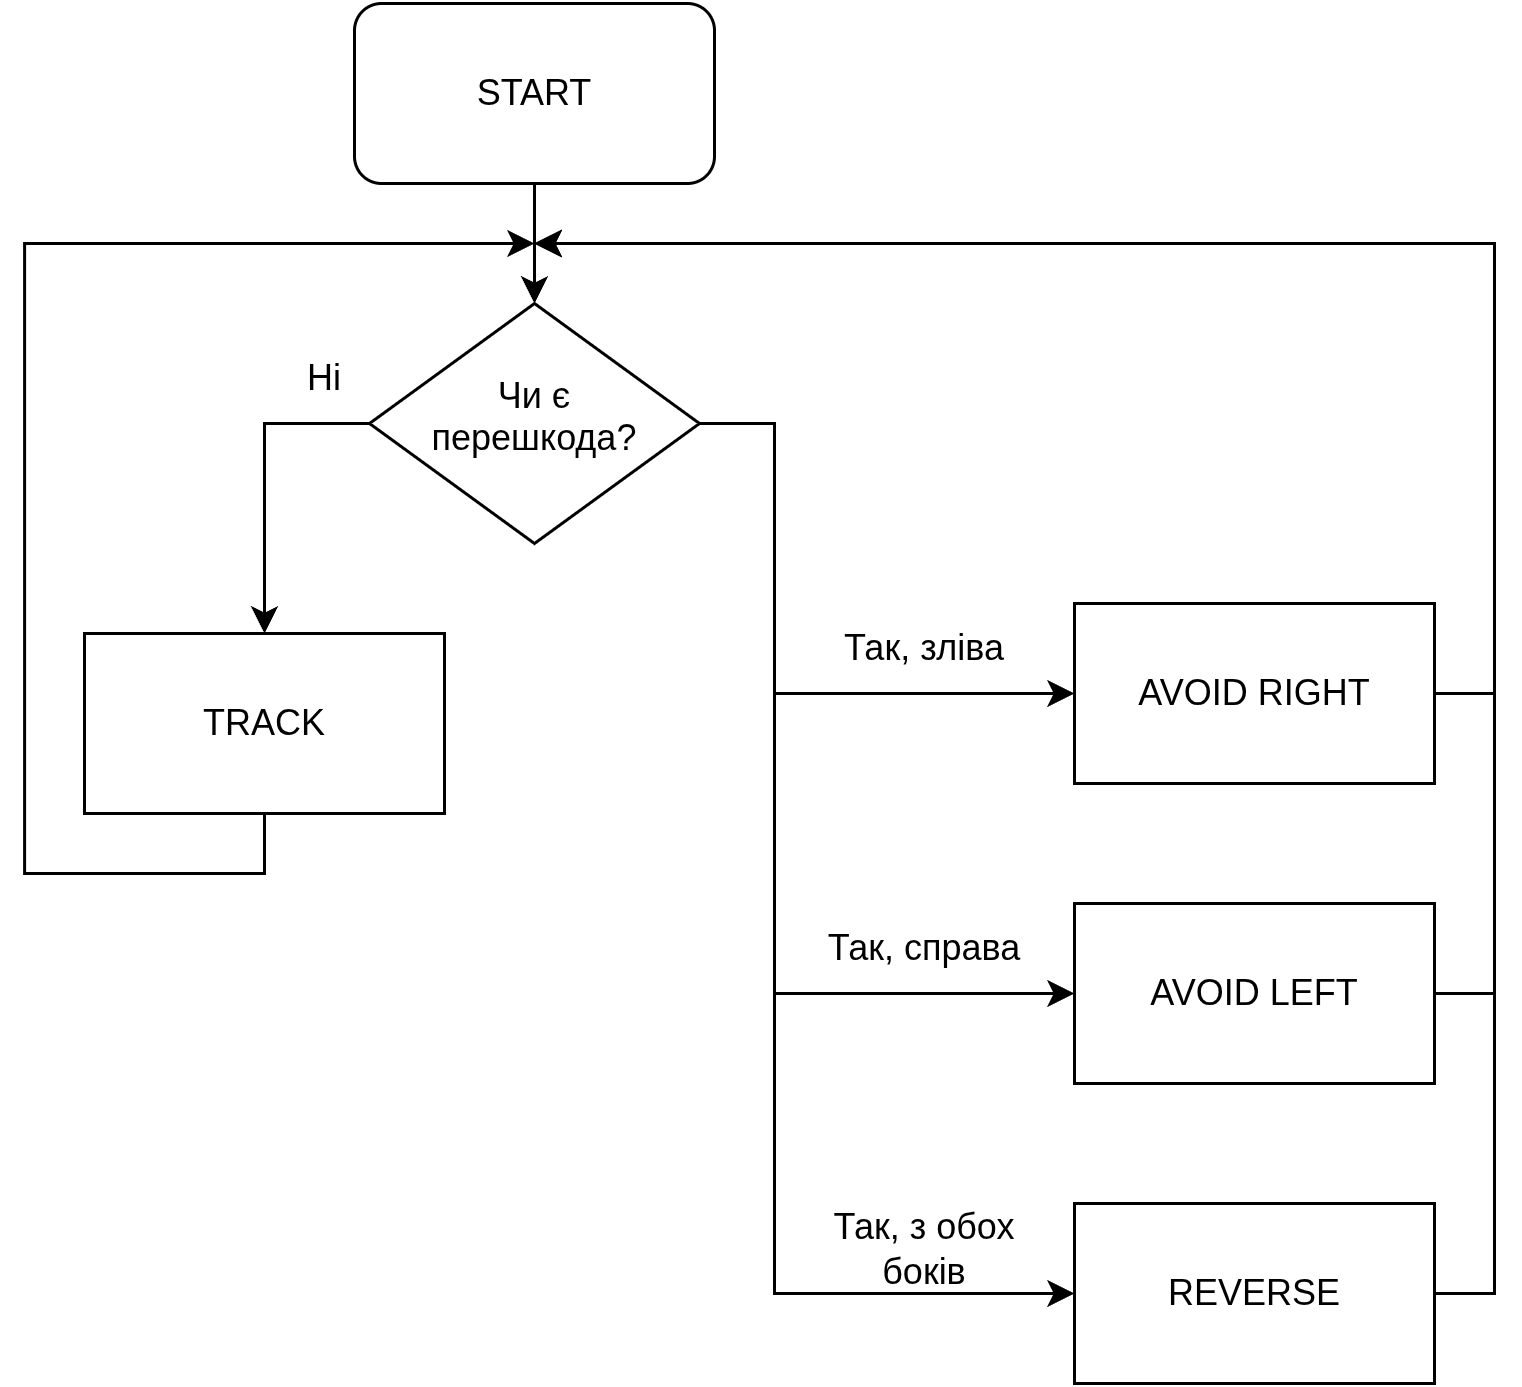
\includegraphics[width=0.86\textwidth]{flowchart.png}
\caption{Циклічний алгоритм реактивного уникнення перешкод}
\end{figure}

\noindent\textbf{Призначення блоків алгоритму.}
\begin{description}[style=nextline,leftmargin=34mm,font=\normalfont\ttfamily]
  \item[START] Початок роботи контролера та перший перехід до опитування сенсорів.
  \item[Чи є перешкода?] Зчитування груп лівих і правих сенсорів та порівняння
  мінімальної відстані з порогом $d_{safe}$.
  \item[TRACK] Обидва колеса отримують однакову додатну швидкість, тому робот
  рухається прямо.
  \item[AVOID RIGHT] Перешкода зліва: робот повертає праворуч різницею
  швидкостей коліс.
  \item[AVOID LEFT] Перешкода справа: робот повертає ліворуч.
  \item[REVERSE] Перешкоди з обох боків: робот рухається назад $0.7$ с,
  після чого повертає у бік з більшою виміряною вільною відстанню.
\end{description}

\section{Програмна реалізація}

Функція \texttt{group\_distance} обчислює мінімальну відстань у заданій
групі сенсорів. Функція \texttt{turning} обирає реакцію, а
\texttt{proc} реалізує стани руху, від'їзду та повороту. Для кожного
робота зберігаються власний стан і час його завершення.

\inputminted[firstline=15,lastline=100]{python}{../src/main.py}

\section{Результат виконання}

\begin{figure}[H]
\centering
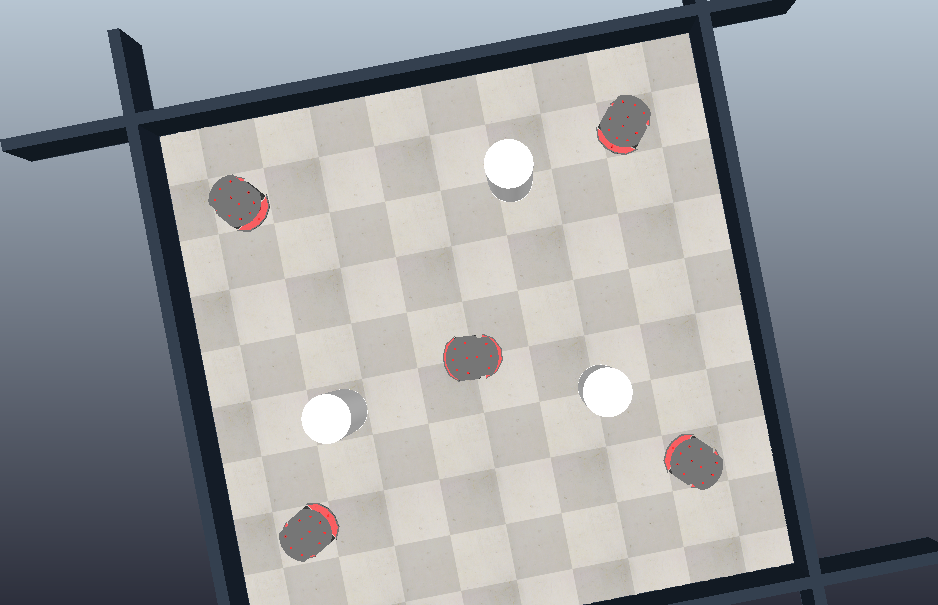
\includegraphics[width=0.84\textwidth]{current_scene.png}
\caption{Актуальна сцена з мобільними роботами, циліндричними перешкодами
та огорожею арени у CoppeliaSim}
\end{figure}

У сцені одночасно працюють п'ять Pioneer P3-DX. Вони мають окремі покази
сенсорів та власний стан автомата, але використовують однаковий алгоритм.
Перешкодами є стіни арени, циліндри та інші роботи. За зміни стану програма
виводить у консоль CoppeliaSim повідомлення через \texttt{sim.addLog}.

\section{Висновок}

Створено замкнену систему керування групою мобільних роботів Pioneer P3-DX.
Програма Python через ZeroMQ Remote API читає дані ультразвукових сенсорів
і задає швидкості приводів. Використання руху назад з наступним поворотом
дозволяє вийти із ситуації, коли перешкоди виявлено з обох боків.
\end{document}
